\xchapter{Proposta do trabalho}
{ }%trata-se  da  apresentação  do  estado  em   que  se encontra  o  projeto, dissertando quais são as contribuições esperadas, seguido pelo cronograma de atividades}

% \presetkeys%
%      {todonotes}%
%     {inline,backgroundcolor=yellow}{}

O \ac{SAD} caracteriza-se como uma modalidade de atenção à saúde composta por um conjunto de ações de prevenção, reabilitação e tratamento de doenças prestadas em domicílio.
Esse serviço tem se tornado cada vez mais presente como ação de saúde complementar ou substituto à internação hospitalar, pois oferece uma nova modalidade de atendimento às pessoas com quadro clinico estável que necessitam de cuidados.
Essa modalidade permite maior comodidade aos pacientes, aumentando o conforto e facilitando o apoio familiar, além de auxiliar a reduzir os riscos contaminação hospitalar e reduzir a lotação nos hospitais. 
A \ac{FESFSUS} é um órgão público, sem fins lucrativos que tem como uma das suas atribuições oferecer serviço de atenção domiciliar a pacientes com médio ou alto grau de complexidade.

O roteamento e escalonamento da equipe de internação domiciliar ainda é realizado de forma manual no Brasil e em diversos países, por vezes utilizando mais tempo do que o esperado na tarefa de elaborar o escalonamento e o roteamento das equipes e em alguns casos gerando resultados ineficazes.

Acredita-se que a partir da utilização de heurísticas para a elaboração de escalas de trabalho, e das rotas, serão gerados resultados mais eficientes, e como consequência será possível aumentar a cobertura do programa, assim como sua visibilidade, permitindo a expansão do atendimento a pacientes com baixa complexidade e o aumento o total de pacientes de média ou alta complexidade atendidos.  

\section{Resultados esperados}

Como resultados esperados após o fim da pesquisa, temos:

\begin{itemize}
\item Revisão sistemática de literatura, permitindo uma discussão sobre heurísticas aplicadas ao \ac{SAD} e auxiliando no processo de obtenção de materiais para pesquisas futuras;
\item Metodologia detalhada do experimento, garantindo a reprodutibilidade em trabalhos futuros;
\item Solução heurística para o problema do \ac{FESFSUS} que pode ser adaptada para utilização em outros casos específicos e utilizada em casos gerais;
\end{itemize}

\section{Metodologia e Métodos}

A metodologia utilizada neste projeto levará em consideração abordagens heurísticas e técnicas de teoria dos grafos, além de um estudo de caso e pesquisa qualitativa e quantitativa.
A seguir serão analisadas algumas abordagens heurísticas, sendo uma delas utilizadas para basear a construção de uma nova heurística para o \ac{SAD}. 

% \subsection{Heurística gulosa}

% Algoritmos gulosos sempre escolhem a melhor solução para o momento partindo do ótimo local em busca do ótimo global. Apesar deste algoritmo encontrar a solução ótima para vários problemas, nem sempre é possível alcançar a solução ótima a partir da execução deste algoritmo~\cite{Cormen:2009}. 

% Em um algoritmo guloso, a cada iteração, um novo elemento do conjunto solução é incorporado à construção da solução parcial até que a solução completa seja obtida. A seleção do próximo elemento que será incorporado é determinado a partir da função gulosa de avaliação. Essa função gulosa representa o aumento incremental na função custo para a incorporação deste elemento na solução parcial em construção~\cite{resende:2014}. O critério para estabelecer qual elemento será selecionado é o do elemento menos custoso, como podemos ver no algoritmo~\ref{guloso}. 

% \begin{algorithm}[H]
%  \Entrada{$C \neq \emptyset$} //conjunto de candidatos \\
%  \Saida{melhor solução segundo o critério guloso}
%    \Inicio{
%    		$S \longleftarrow \emptyset $ \mbox{//o conjunto solução $S$ está vazio inicialmente} \\
%         $C \longleftarrow E $ \mbox{//inicializa o conjunto $C$ com o conjunto inicial $E$} \\
%      \While {$C \neq \emptyset \wedge \neg solucao(S)$ }{
%         $ x \longleftarrow seleciona(C)$ \mbox{//seleciona o proximo candidato} \\
%         $C \longleftarrow C - x$ \mbox{//remove x do conjunto de candidatos} \\
%         \eIf{Viavel($S + x$)}{
%         	$S \longleftarrow S + x$  \mbox{//adiciona o candidato ao conjunto solucao}\\
%         }{$S \longleftarrow S$} \mbox{//nao atualiza o conjunto solucao} \\
%      }
%      \Retorna{S} \mbox{//melhor solução segundo o critério guloso} \\
%    }
%  \caption{Algoritmo guloso}
%  \label{guloso}
% \end{algorithm}

%\subsection{Greedy Randomized Adaptative Search procedure - GRASP}

%O GRASP é uma heurística gulosa adaptativa de randomização iterativa constituída por duas fases: Uma fase construtiva e outra fase de busca local~\cite{feo:1995} e~\cite{resende:2014}.

%Para descrever o GRASP será levado em consideração o problema de otimização combinatorial para minimizar a função $f(s)$ para cada solução $S \in X$, sendo definido a partir de um conjunto inicial finito $E = \{ e1, e2, ..., en \}$ para um conjunto viável de um conjunto soluções viáveis $X \subseteq 2^E$ e pela função objetiva $f:2^E \leftarrow R$. 
%O conjunto de soluções viáveis para o problema é definido a partir do E, a função objetivo e das restrições~\cite{resende:2014}.

%Na fase de construção é elaborada uma solução, se esta solução não for viável, esta é descartada ou é aplicada uma heurística reparatória para alcançar a viabilidade. Uma vez que a solução viável é obtida, a vizinhança que possui a solução é investigada até que seja encontrado o mínimo local através da etapa de busca local. Levando em consideração que o GRASP é uma heurística gulosa, não é garantido que a solução ótima será encontrada todas as vezes a partir do ótimo local~\cite{resende:2014}.

%A heurística adaptativa é chamada dessa forma porque os benefícios associados com cada elemento é atualizado a cada iteração da fase construtiva para refletir as mudanças trazidas pela seleção do elemento anterior.

%Para a elaboração da etapa construtiva, na qual solução viável é construída iterativamente, um elemento por vez e a cada iteração a escolha do próximo elemento que será adicionado é determinado pela ordem de todos os elementos candidatos em uma lista que respeita a função gulosa, são utilizados algoritmos randomizados.
%Os algoritmos randomizados são importantes para gerar o espaço de busca inicial em uma vizinhança, quebrar loops, habilitar trajetórias diferentes para seguir em uma mesma solução inicial ou simplificar diferentes partes em uma vizinhança extensa. 
%Na fase de busca local, é utilizado um algoritmo de busca local que funciona de maneira iterativa, substituindo sucessivamente a solução corrente pela melhor solução encontrada na vizinhança, determinando quando a melhor solução não é encontrada na vizinhança ~\cite{resende:2014}.


%\subsection{Adaptative Iterated Construction Search}
%não tem artigos falando sobre

%O \ac{AICS}, assim como o \ac{GRASP}, é um algoritmo utilizado para resolver problemas de otimização, pertencente à sub-área de otimização estocástica, ou seja, o conjunto de soluções viáveis que é ou pode ser reduzido a um conjunto discreto. Esse algoritmo utiliza a experiência adquirida em soluções passadas para gerar soluções melhores. Uma forma de implementar esta ideia é associar pesos com possíveis decisões que serão tomadas durante o processo construtivo. Estes pesos são adaptados através de múltiplas iterações do processo de busca para refletir a experiência de iterações passadas \cite{hoss:2005}.

\subsection{Constraint Programming}

O problema de satisfação de restrição, consiste em um conjunto finito de variáveis, sendo que cada variável está associada a um valor e a um conjunto de restrições.  A solução para o problema de satisfação por restrição é a satisfação de todas as restrições do domínio~\cite{maria:2008}.

A programação por restrições lógicas é uma extensão da programação lógica, sendo ambas consideradas pertencentes ao paradigma declarativo, dessa forma o programador foca em o que computar ao invés de como computar. neste método possui um conjunto finito de regras cujo corpo contem conjunções de literais, simbolo atômicos e restrições de domínio~\cite{maria:2008}.

%\subsection{Variable Neighborhood Search}

%O \ac{VNS} explora uma vizinhança de forma a chegar cada vez mais distante da solução atual, trocando a solução atual por uma nova, se e somente se, a melhoria já foi feita, dessa forma, características de uma solução cuja varias variáveis já possuem seu valor ótimo, serão mantidas e usadas para obter uma boa vizinhança~\cite{hansen:2001}.

%Seja $N_{k} = (1, 2, ..., k_{max}) $ um conjunto finito de estruturas de vizinhanças pré selecionadas, $N_{k}(x)$ um conjunto solução da vizinhança $k$ de $x$. A condição de parada é a máxima capacidade da CPU, o maior número de iterações, o a maior quantidade de iterações entre duas melhorias. Geralmente, sucessivas vizinhanças $N_{k}$ estão aninhadas~\cite{hansen:2001}.

\section{Atividades previstas}
%trata-se   da   explicitação   do   modo   como  será desenvolvido o trabalho
Como foi visto anteriormente, existem várias abordagens heurísticas para o problema de escalonamento e roteamento do \ac{SAD}, sendo que algumas dessas heurísticas foram aplicadas a casos específicos. Nesse contexto, foi levantada a hipótese de que é possível elaborar uma abordagem heurística para o problema de roteamento e escalonamento do Serviço de Atendimento Domiciliar em Salvador, prestado pela \ac{FESFSUS}.

Para validar a nossa hipótese um estudo de caso com o Serviço de Atendimento Domiciliar em Salvador, a \ac{FESFSUS}, em busca de verificar e analisar as suas principais necessidades.

Foi realizada uma revisão sistemática de literatura para levantar quais abordagens heurísticas que estão sendo utilizadas atualmente para solucionar o problema de escalonamento e roteamento do \ac{SAD}, e dessa forma, a partir do entendimento de casos já estudados tratar o caso da \ac{FESFSUS} e posteriormente casos mais gerais.

Após o estudo de diversas abordagens levantadas e elaboração da abordagem heurística, serão utilizados dados do próprio projeto estudado, e para complementar o trabalho, além de bases de dados publicadas gratuitamente na web, contendo informações relevantes à pesquisa.

A partir da pesquisa realizada no caso específico da cidade de Salvador e dos experimentos realizados com o grupo \ac{FESFSUS}, buscamos gerar uma nova heurística que após algumas adaptações, também possa também ser utilizada em casos gerais.

\subsection{Cronograma de atividades}

O cronograma seguinte apresenta o desenvolvimento das atividades executadas desde o início da pós-graduação, tendo as atividades representadas a cada mês levado em consideração um curso com duração de 24 meses, com início em Novembro de 2016 e final previsto para Novembro de 2019, no qual as disciplinas obrigatórias e optativas, assim como o estágio docente orientado foram realizados no primeiro ano de curso, como pode ser visto na seguinte figura \ref{cronograma_atividade}.

%cronograma de atividades
\begin{figure}[H]
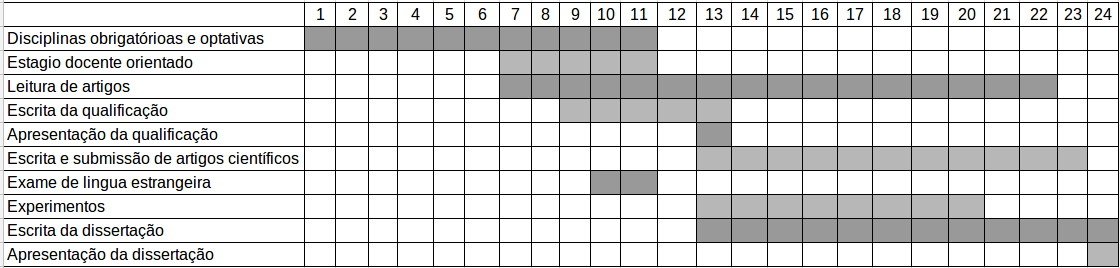
\includegraphics[width=1 \textwidth]{cronograma_atividades.png}
\begin{center}
\caption{Cronograma de atividades \label{cronograma_atividade}}
%Fonte: Elaborada pelo autor
\end{center}
\end{figure}

